\section{Choque}

\subsection{Hipótese de Newton}

Assumindo a Hipótese de que as superfícies dos corpos nas quais ocorre o choque são lisas, podemos afirmar que apenas a velocidade projetadas na normal de choque sofrerão alteração

\begin{center}
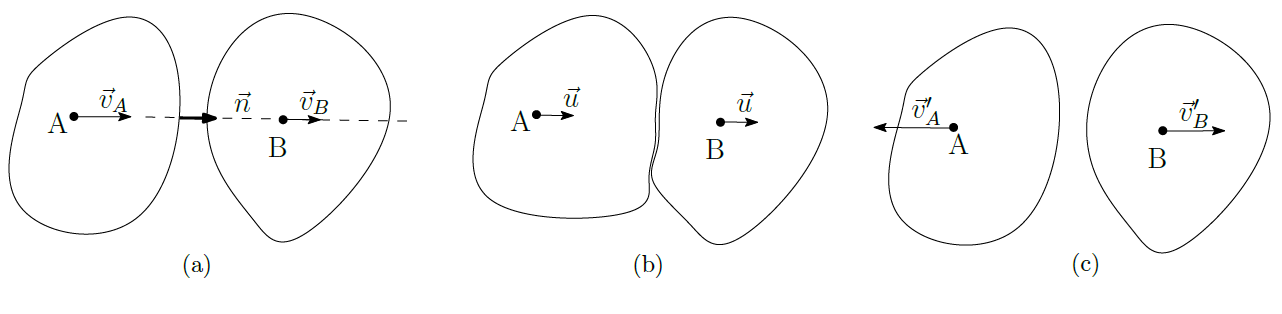
\includegraphics[width=8cm]{C:/Users/patri/Downloads/Poli/lateco/mecanica/figuras/hipotese_choque.png}
\end{center}

Na Hipótese de Newton define-se um \textit{coeficiente de restituição} que é a proporção entre as velocidades do centro de massa dos corpos anteriormente ao choque e posteriormente ao choque

$$ \boxed{V_A' - V_B' = e(V_B - V_A)} $$

O valor deste coeficiente determina o tipo do choque estudado.

\begin{enumerate}
	\item $e = 1$, choque perfeitamente elástico
	\item $0 < e < 1$, choque parcialmente elástico
	\item $e = 0$, choque inelástico
\end{enumerate}

\subsection{Hipótese de Poisson}

A etapa de Poisson divide o choque em duas etapas

\begin{enumerate}
	\item Etapa de Compressão. Haverá compressão das superfície até que as forças Impulsivas igualem as velocidades dos pontos de contato.
	\item Etapa de Restituição. As superfícies se expandem e os corpos se separam.
\end{enumerate}

\begin{center}
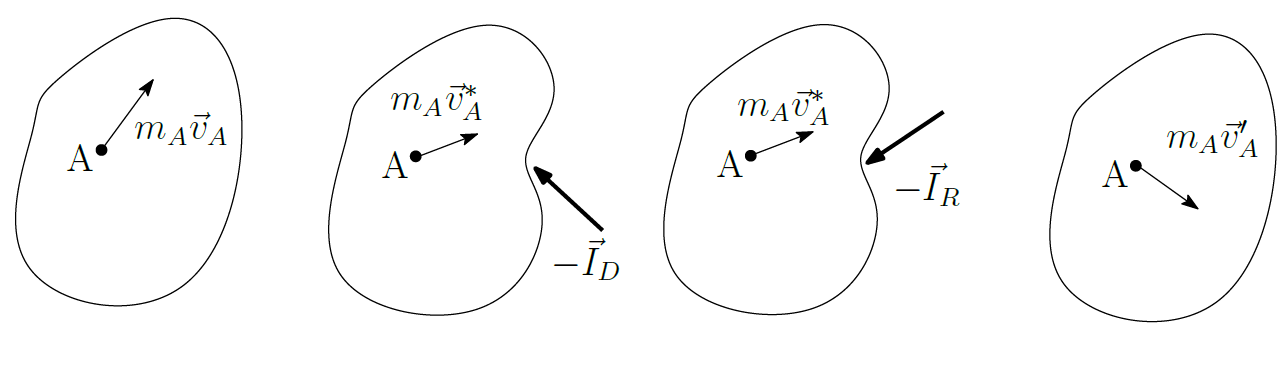
\includegraphics[width=8cm]{C:/Users/patri/Downloads/Poli/lateco/mecanica/figuras/choque_poisson.png}
\end{center}

Onde a direção dos Impulsos sempre será à da normal de choque caso as superfícies sejam adotadas como lisas.

Esta hipótese utiliza do \textit{coeficiente de restituição} para estabelecer a relação entre as velocidades antes do choque e posteriores ao choque.

$$ \boxed{e = \frac{\vec{I_r}\cdot \vec{n}}{\vec{I_D}\cdot \vec{n}} = \frac{V_A' - V_B'}{V_B - V_A}} $$